\newpage

\section{Структура НКИ}
{\bf Нейрокомпьютерные интерфейсы (НКИ)} - это устройства которые позволяют получать информацию об активности мозга, анализировать и переводить её в понятный для компьютера машинный код(двоичный), таким образом становится возможным управлять внешними устройствами, начиная с курсора мыши, заканчивая полноценными экзоскелетами. 

 НКИ не считывает сигналы с мышц. Основная цель НКИ заключается в замене или восстановлении функций людям, которые утратили их в силу нервно-мышечных расстройств, таких как боковой амиотрофический склероз \footnote{заболевание ЦНС, при котором происходит поражение двигательных нейронов.}, церебральный паралич\footnote{ группу нарушений двигательных функций мозга.}, инсульт или повреждение спинного мозга. Начиная с простейших устройств, исследователи продолжали использовать электроэнцефалографические, внутрикортикальные, электрокортикографические и другие сигналы мозга для все более сложного контроля над различными устройствами. 
 
 Стоит отметить, что НКИ используется не только на больных людях, она также находит применения и среди здоровых людей. Эта технология приковывает все больше внимания со стороны научного сообщества. Она интересна как инженерам, так и  биологам, химикам, физикам, хирургам, физиологам и.т.д. За последние 15 лет наблюдается очень большой рост исследований, публикуется все больше работа на эту тему, это видно на рис. \ref{papers}
  
 Для дальнейшего развития технологии важно учесть следующие составляющие . 
 
 \begin{itemize}
 	\item Интерфейсы, управляемые компьютером, требуют оборудования для сбора сигналов. Оно должно быть удобным, безопасным, легким для перемещения.
 	\item НКИ необходимо проверять в долгосрочных исследованиях. Это нужно для широкого распространения этой технологии
 	\item Необходимо повышать надежность НКИ и скорость отклика. 
 \end{itemize}

\begin{figure}[h]
	\center	{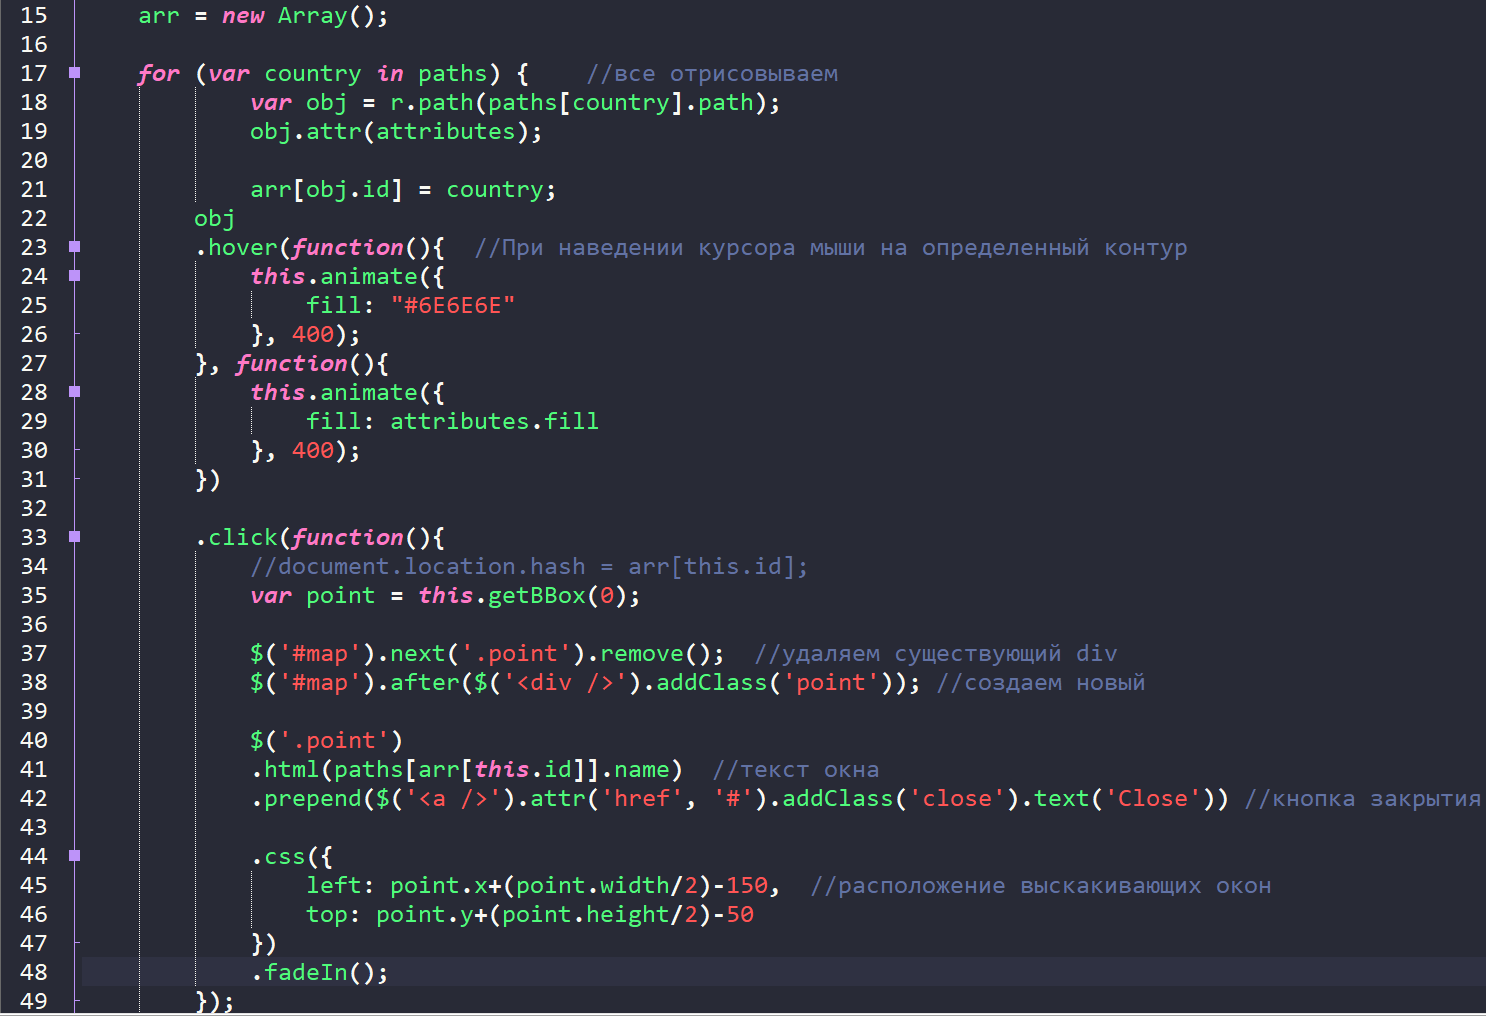
\includegraphics[scale=0.6]{6}}
	\caption{Количество исследований, связанных с технологией НКИ. Информация взята с ресурса pubmed.com}
	\label{papers}
\end{figure} 



\subsection*{История НКИ}
Первая попытка контролировать сигналы мозга человека на нейрофизиологической основе была предпринята в 1969 году. Камия с коллегами показал, что здоровый человек способен обучиться изменять $\alpha$-ритм\footnote{колебания активности нейронов, регистрируемые с помощью ЭЭГ} в своем мозге, при непрерывной обратной связи, показывающий активность в данный момент времени. Также велись работы над коммуникацией, над системами позволяющими вводить текст, использовалась ЭЭГ.

Прорывом в области НКИ можно считать использование инвазивных систем. То есть электроды, устанавливаются непосредственно в кору мозга.

Так Кеннеди со своими коллегами первыми сконструировали внутрикорковый НКИ. Они имплантировали электроды непосредственно внутрь затылочной коры обезьяны.
Спустя несколько лет Дан смог проделать тоже самое на кошках. В результате обработки информации, он получил изображения того, что видит животное в данный момент. Такие же исследования были проведены над людьми \cite{image}, правда стоит отметить, что не применялось хирургическое вмешательство. Использовался другой тип НКИ(неинвазивный). В следующем разделе обозначим различные типы НКИ, используемые учеными.

\section{Различные типы НКИ}
В начале 21 века произошел быстрый прирост исследований в области НКИ. Этот прогресс обусловлен созданием новых и совершенствования старых методов регистрации активности мозга. Также ученые стали регистрировать различные сигналы. Но обо всем по порядку.

НКИ можно поделить на две группы: {\bf инвазивные} и на {\bf неинвазивные}. Суть проста. Для инвазивных систем требуется хирургическое вмешательство, поэтому они более затратны и используются либо на животных, либо на больных людях. А неинвазивные соответственно не требуют никакого вмешательства.

Общий принцип всех НКИ очень схож. Сигналы мозга регистрируются, усиливаются, фильтруются и декодируются. После обработки и декодирования мозговых сигналов, они могут использоваться для управления движением протеза, инвалидного кресла, курсора мыши, а также для электрической стимуляции определенных мышц.

Стоит отметить, что в медицине НКИ классифицируются ещё по одному признаку. Разделяют на те, что помогают в реабилитации больных, и на "ассистивные" (заменяющие утраченные функции). Мы не станем использовать эту классификацию, так как для нас важно разобраться в принципах работы НКИ.  
\subsection*{Инвазивные}
Использование инвазивных систем включает в себя хирургическую имплантацию электродов или много-электродных сеток. Инвазивные НКИ измеряют активность нейронов, с помощью которых наш мозг кодирует повендеческую информация. Например, для управления протезами, электроды устанавливают на кору, отвечающую за движение.

Существует четыре основных типа активности мозга, которые измеряются с помощью инвазивных НКИ: 
\begin{itemize}
	\item локальные полевые потенциалы (LFP)
	\item односекторная активность. Регистрация отдельных потенциалов действия (SUA)
	\item многоузловая активность. совокупность локальных полей (MUA)
	\item электрокортикографический колебания, регистрируемые с поверхности коры (электрокортикография, ECoG)
%	\item проницаемость кальциевых каналов
\end{itemize}
В последние годы ведутся разработки в области эндоваскулярных (внутри сосудов) НКИ \cite{litlink2}. Электроды по сосудам отправляют в нужную зону мозга и регистрируют активность прилежащей части мозга. Исследователи утверждают, что этот способ менее опасен, нежели другие инвазивные систем, однако долгосрочных исследований в данной области не приводилось. 

Инвазивные системы дают очень высокий уровень детализации сигналов, что необходимо для работы с точными движениями. Это огромное преимущество по сравнение с неинвазивными системами нивелируется дороговизной и необходимостью в проведении хирургического вмешательства, а также возможностью заражения, или отторжения устройств. Также не были проведены долгосрочные исследования о влиянии инвазивных средств на здоровье пациента

По этим причинам исследований в этой области не так много, а в России практически нет лабораторий работающих в этом направление. Поэтому я решил более подробно остановиться на неинвазивных НКИ.


\subsection*{Неинвазивные}
Неинвазивные НКИ не требуют хирургической имплантации и позволяют регистрировать сигналы головного мозга с внешней поверхности кожи головы. А метаболические сигналы регистрируются в самом мозге, однако необходимые устройства устанавливаются на поверхности кожи В общем, эти интерфейсы в зависимости от задачи регистрируют пять типов сигналов мозга. 
\begin{itemize}
	\item Электрические сигналы.
	\begin{itemize}	
		\item Сенсоромоторные ритмы. О них речь уже заходила. Человек может научиться управлять ритмами, тем самым управлять системой
		\item Медленные корковые потенциалы. Эти потенциалы регистрирует обычные ЭЭГ. Также как сенсоромоторными ритмами, человек может ими управлять
		\item P300 связанный с событием потенциал.  Через 300 мс после неожиданного стимула наблюдается потенциал, который можно регистрировать с помощью ЭЭГ
	%	\item Устойчивые визуальные вызванные потенциалы. 
	%	\item Связанные с ошибкой отрицательные вызванные потенциалы	
	\end{itemize}
	\item Метаболический уровень (BOLD)
	\begin{itemize}	
	\item Уровень кислорода в крови. Речь идет об использовании функциональной МРТ для детектирования изменения метаболической активности мозга
	\item Уровень кислорода в крови. Используется cпектроскопия в ближней инфракрасной области(БИК)
	\end{itemize}
\end{itemize} 

Неинвазивные системы более распространены, так как не требуется никакого хирургического вмешательства. Однако они не способны дать ту детализацию сигналов, которую дают инвазивные НКИ. Это связано с тем что мы регистрируем активность лишь на кожи головы мозга, и мы не можем знать от куда тот или иной сигнал взялся. Мы наблюдаем лишь некую суммарную активность, которую невозможно использовать для определения точных движений, желаний и.т.д.

Стоит отметить что НКИ основанные на метаболических сигналах, в теории могут дать нужную детализацию, но у них есть другая проблема. Она связанна со скоростью отклика. 

Подробно обо всем этом пойдет речь в следующей главе. Там мы детально остановимся на принципе работы детекторов мозговой активности. Остановимся на рассмотрении основных механизмов

\newpage
Ниже представлена схематичная картина, содержащая в себе почти все системы и наглядно демонстрирующая устройство НКИ.
\begin{figure}[h]
	\center{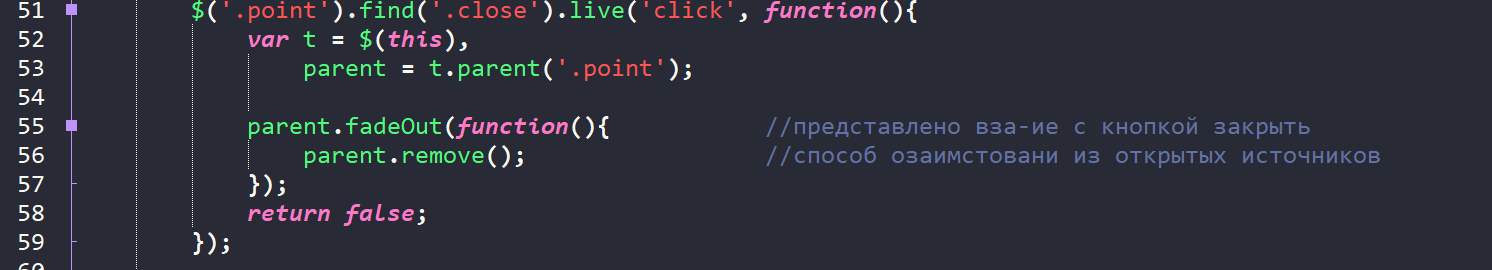
\includegraphics[width=1\linewidth]{7}}
	\caption{Общая картина структуры нейро-компьютерных интерфейсов. Информация взята со следующей статьи\cite{review}}
	\label{fig:image}
\end{figure}
 
